\documentclass[12pt]{article}
\usepackage{graphicx}
\usepackage{psfrag}
\usepackage{epsfig}
\usepackage{subfigure}
\usepackage{amssymb,amsmath}
\usepackage{verbatim}

%\usepackage{doublespace}

\textheight 23cm \topmargin -1cm \leftmargin 0cm

\marginparwidth 0mm    % Largeur des notes marge de droite
\textwidth 16.5cm      % Largeur du texte
\hsize \textwidth      % Longueur d'une ligne
\advance \hsize by -\marginparwidth
\oddsidemargin -4mm    % Marge gauche pages de droite - 1 inch (2.54 cm)
\evensidemargin \oddsidemargin % Idem pour les pages de gauche

\advance\hoffset by 5mm % Pour corriger un decalage residuel sur la gauche

\renewcommand{\hat}{\widehat}
\newcommand{\R}{\mathrm{I\!R\!}}
\newcommand{\C}{\mathrm{I\!\!\!C\!}}
\newcommand{\sinc}{\mbox{sinc}}
\newcommand{\diag}{\mbox{diag}}
\newcommand{\Tr}{\mbox{Tr}}

% commands
\newtheorem{theo}{Theorem}
\newtheorem{proposition}{Proposition}
\newcommand{\nc}{\newcommand}
\nc{\RR}{\mbox{\rm I$\!$R}} \nc{\dsp}{\displaystyle}
\nc{\Div}{\mbox{\rm div }} \nc{\beequ}{\begin{equation}}
\nc{\barr}{\begin{array}} \nc{\earr}{\end{array}}
\nc{\eequ}{\end{equation}} \nc{\BFF}{\hbox{\boldmath{${\cal
F}$}}^{(j)}({\bf y}^s,t)}

\nc{\hr}{\widehat{r}} \nc{\hh}{\widehat{h}} \nc{\hs}{\widehat{s}}
\nc{\hn}{\widehat{n}} \nc{\hw}{\widehat{w}} \nc{\hd}{\widehat{d}}
\nc{\hG}{\widehat{\Gamma}} \nc{\om}{\omega} \nc{\yy}{{\bf y}}
\nc{\ys}{{\bf y}^s} \nc{\yo}{{\bf y}_0} \nc{\xp}{{\bf x}_p}
\nc{\xr}{{\bf x}_r} \nc{\co}{{\cal O}}
\renewcommand\labelenumi{\alph{enumi})}
\begin{document}
\begin{center}
\textbf{Practice Set 2 Solutions}
\end{center}
\paragraph{Problem 1}
Use the following equations to solve the problem.
\begin{eqnarray*}
C_{SIMO} &=& \log (1 + \frac{E_s}{N_o} \sum_{j=1}^{M_R} \|h_j\|^2)\\
C_{MISO} &=& \log (1 +  \frac{E_s}{M_T N_o}\sum_{j=1}^{M_T} \|h_j\|^2)
\end{eqnarray*}
Solutions are $C_{SIMO}=7.6726$ and $C_{MISO}=6.6797$
\paragraph{Problem 2}
Use the following equations to solve the problem.
\begin{eqnarray*}
 C_{MIMO} = \log_2\det\left({\bf I}_{M_R}+\frac{E_s}{M_TN_o}{\bf HH}^H \right)
\end{eqnarray*}
Solution is $C_{MIMO}=14.8927$ 
\paragraph{Problem 3}
\verbatiminput{cdf.m}
See Figure~\ref{fig:cdf} for output.
\begin{figure}
    \centering
  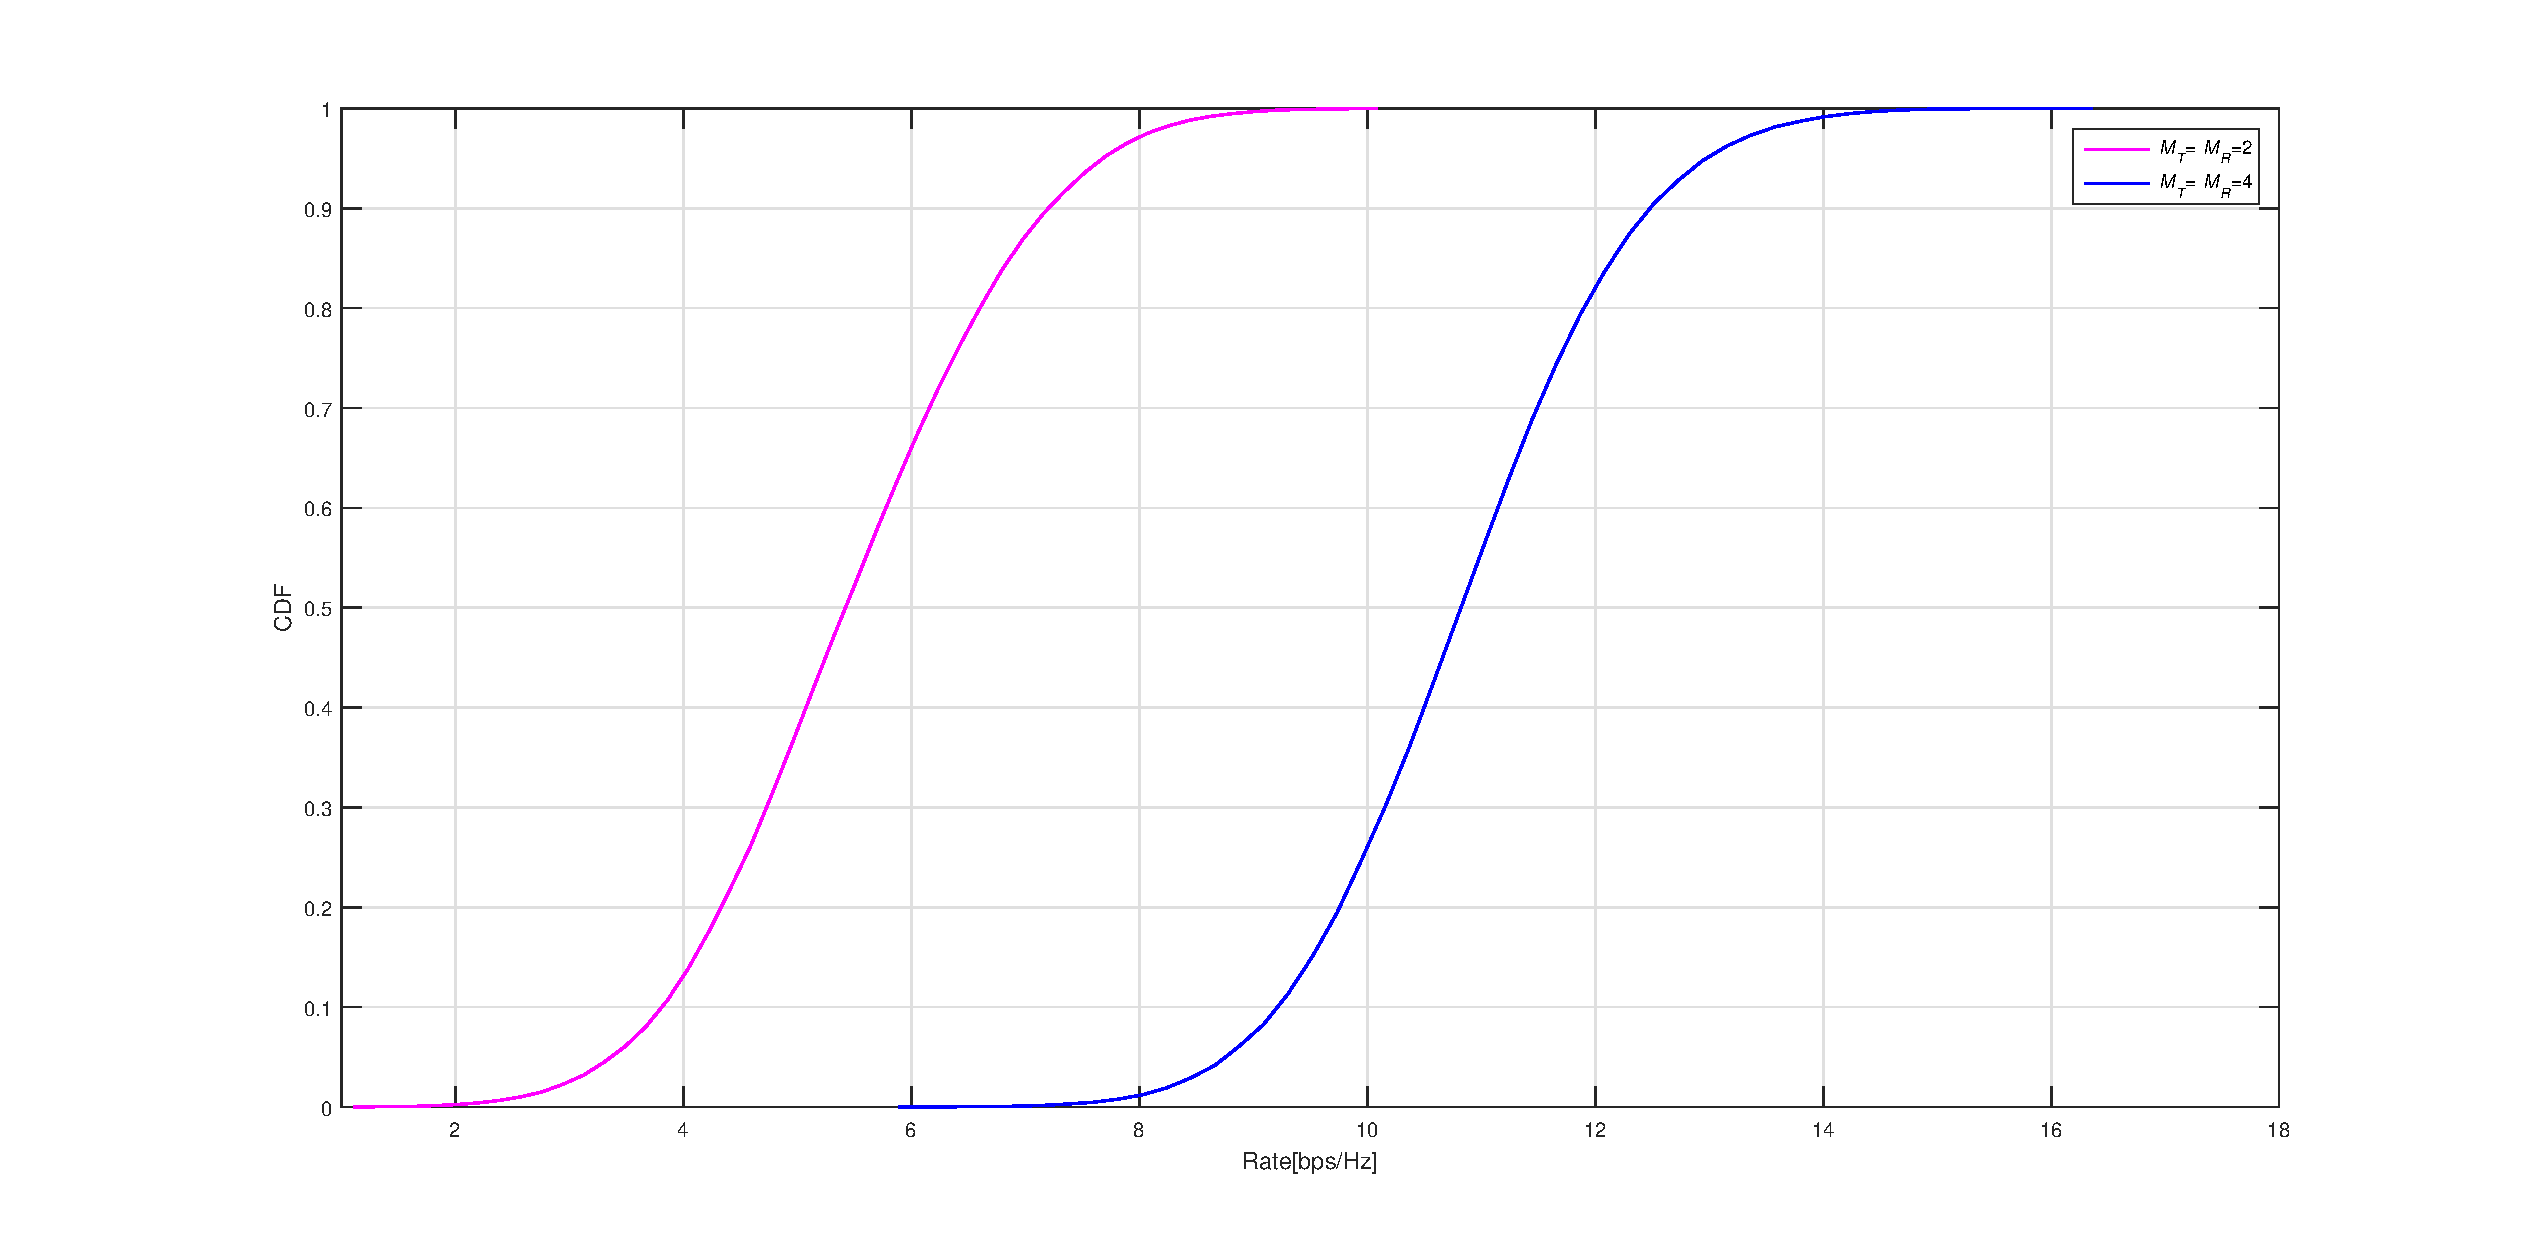
\includegraphics[width=6.0in]{cdf.eps}\\
  \caption{CDF}\label{fig:cdf}
\end{figure}
\paragraph{Problem 4}
\verbatiminput{er_cap.m}
See Figure~\ref{fig:er_cap} for output.
\begin{figure}
    \centering
  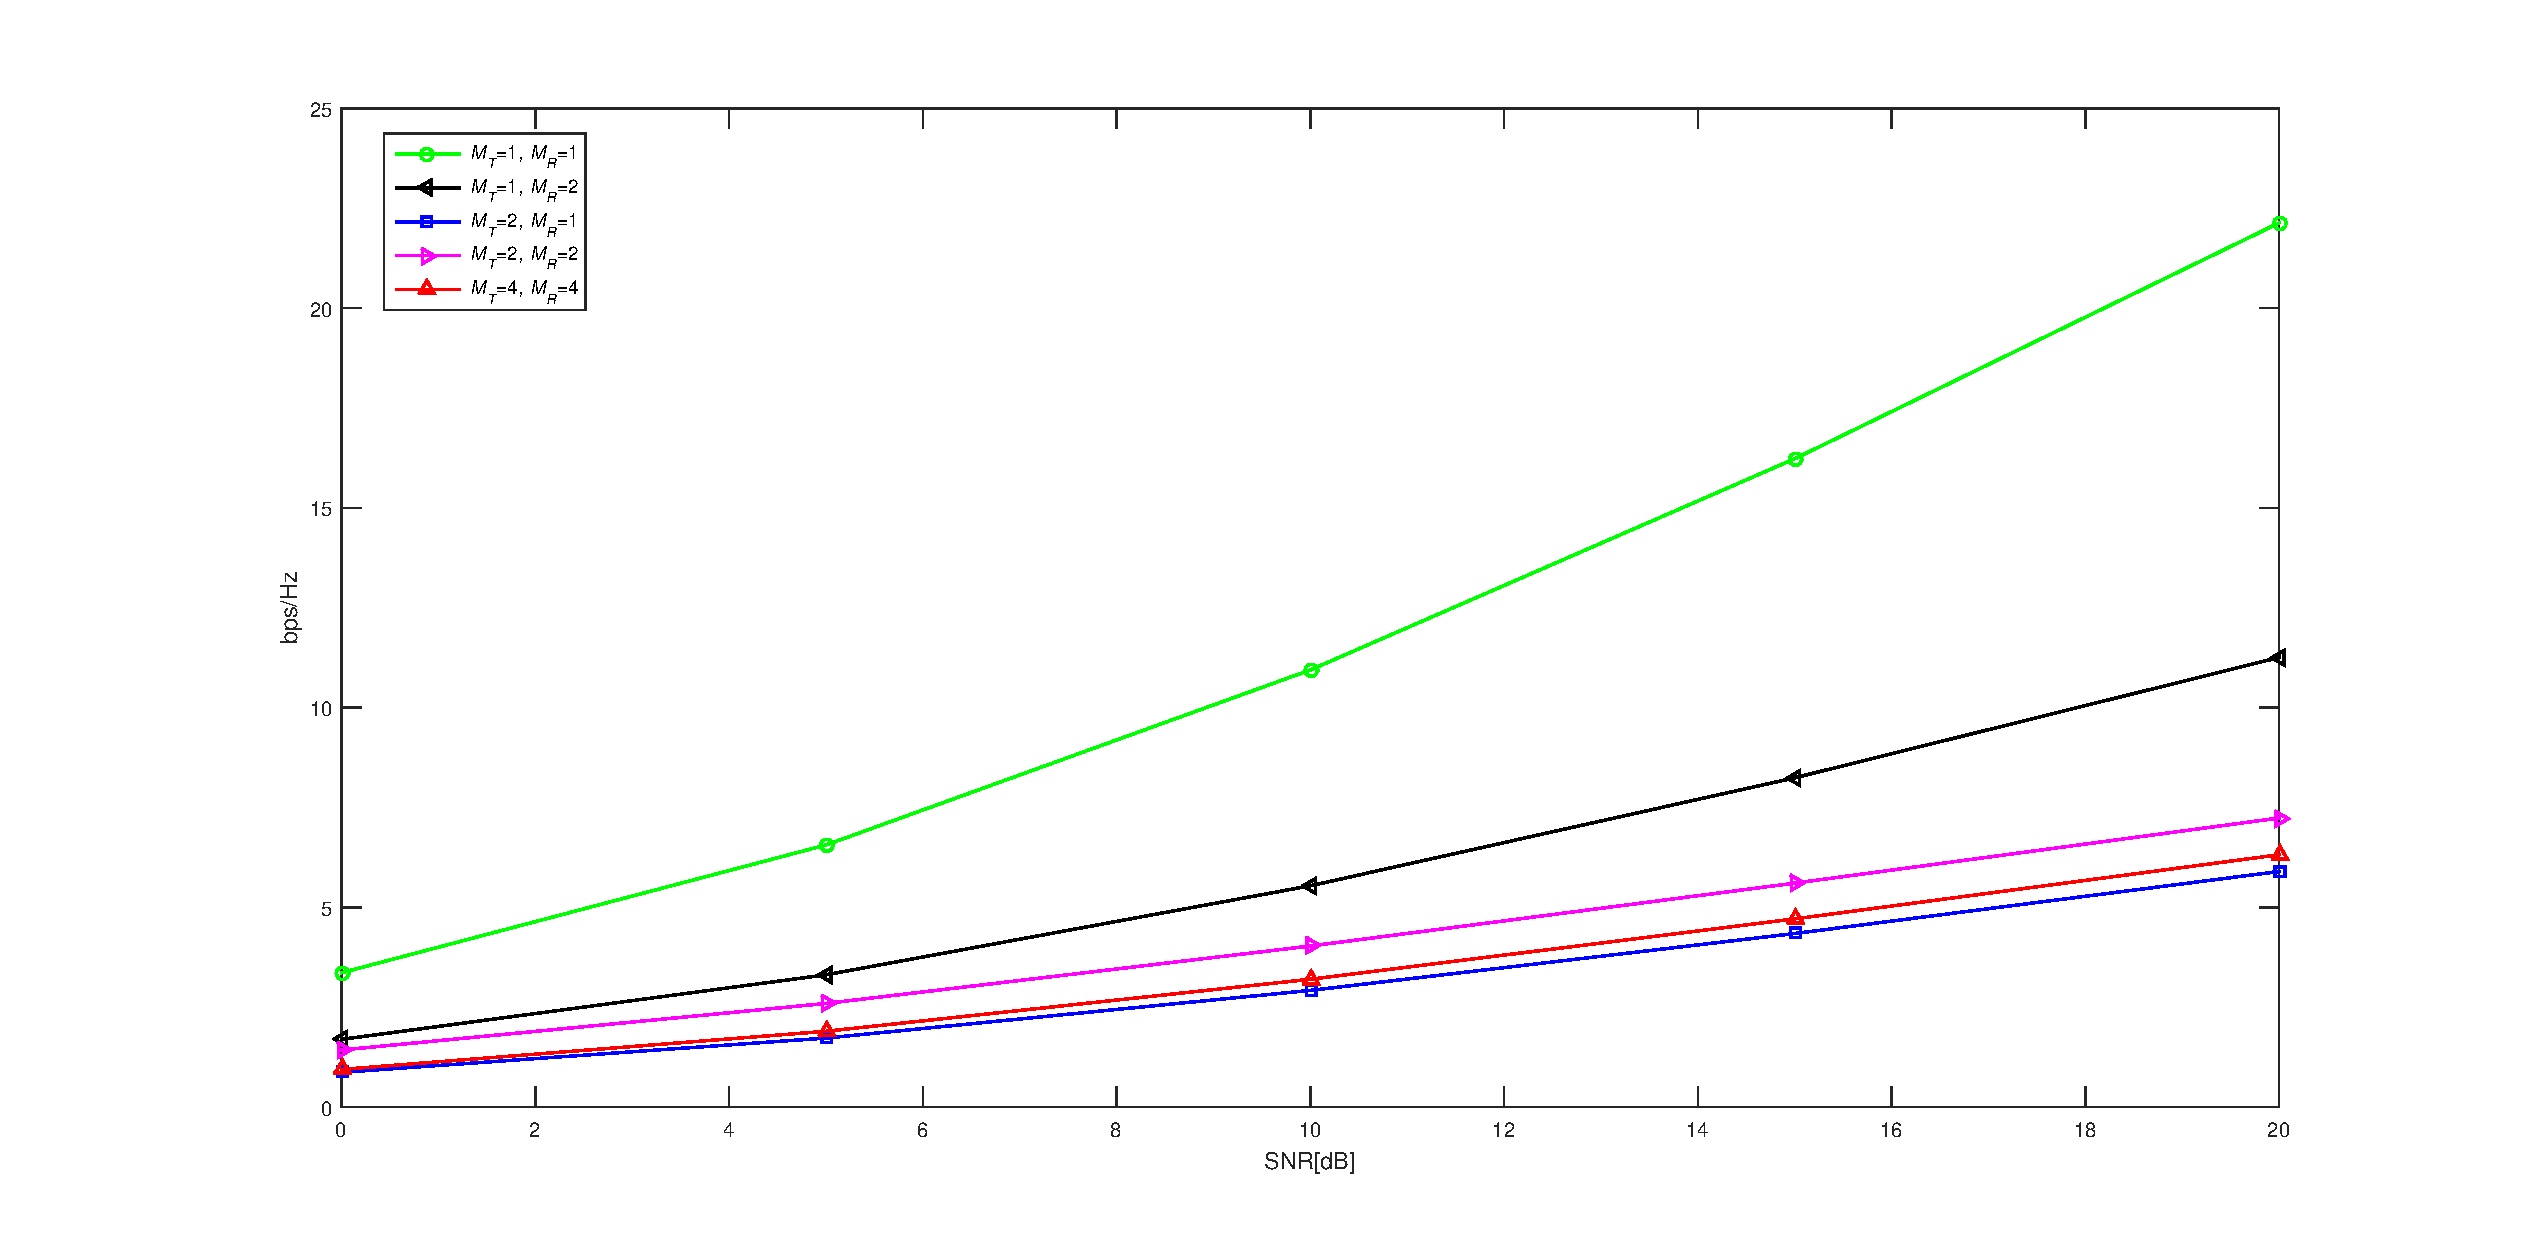
\includegraphics[width=6.0in]{er_cap.eps}\\
  \caption{Ergodic Capacity Vs SNR}\label{fig:er_cap}
\end{figure}
\paragraph{Problem 5}
\verbatiminput{cap_crr.m}
See Figure~\ref{fig:cap_crr} for output.
\begin{figure}
    \centering
  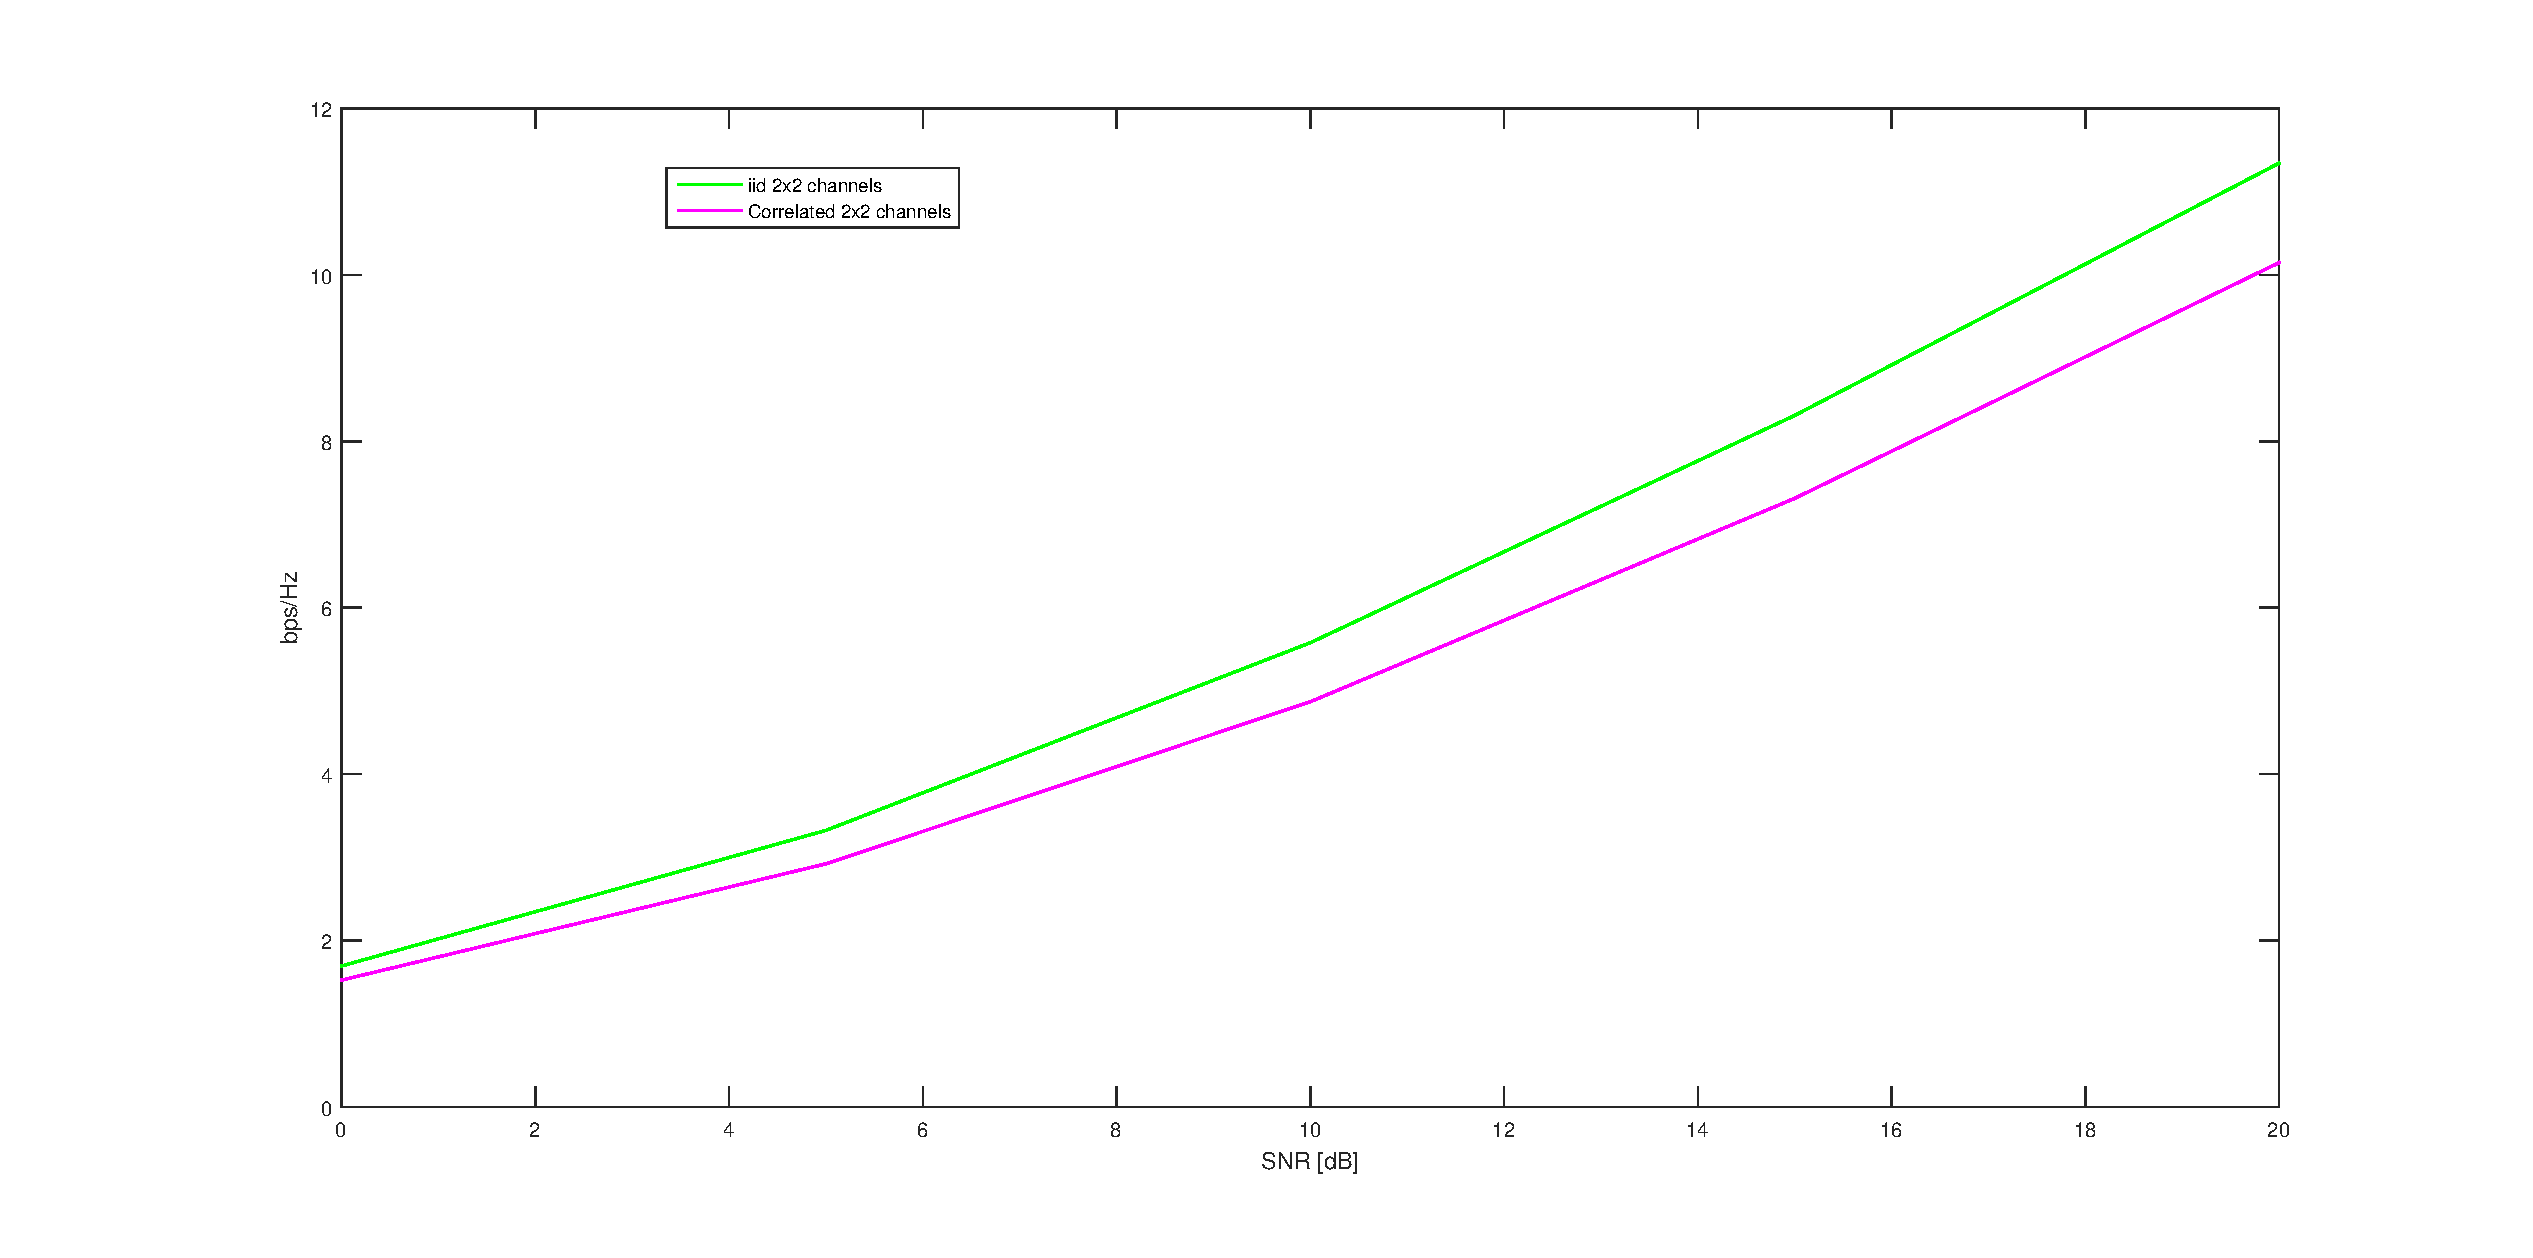
\includegraphics[width=6.0in]{cap_crr.eps}\\
  \caption{Impact of correlated and iid channels}\label{fig:cap_crr}
\end{figure}
\paragraph{Problem 6}
\verbatiminput{mimoRic2.m}
See Figure~\ref{fig:mimoRic2} for output.
\begin{figure}
    \centering
  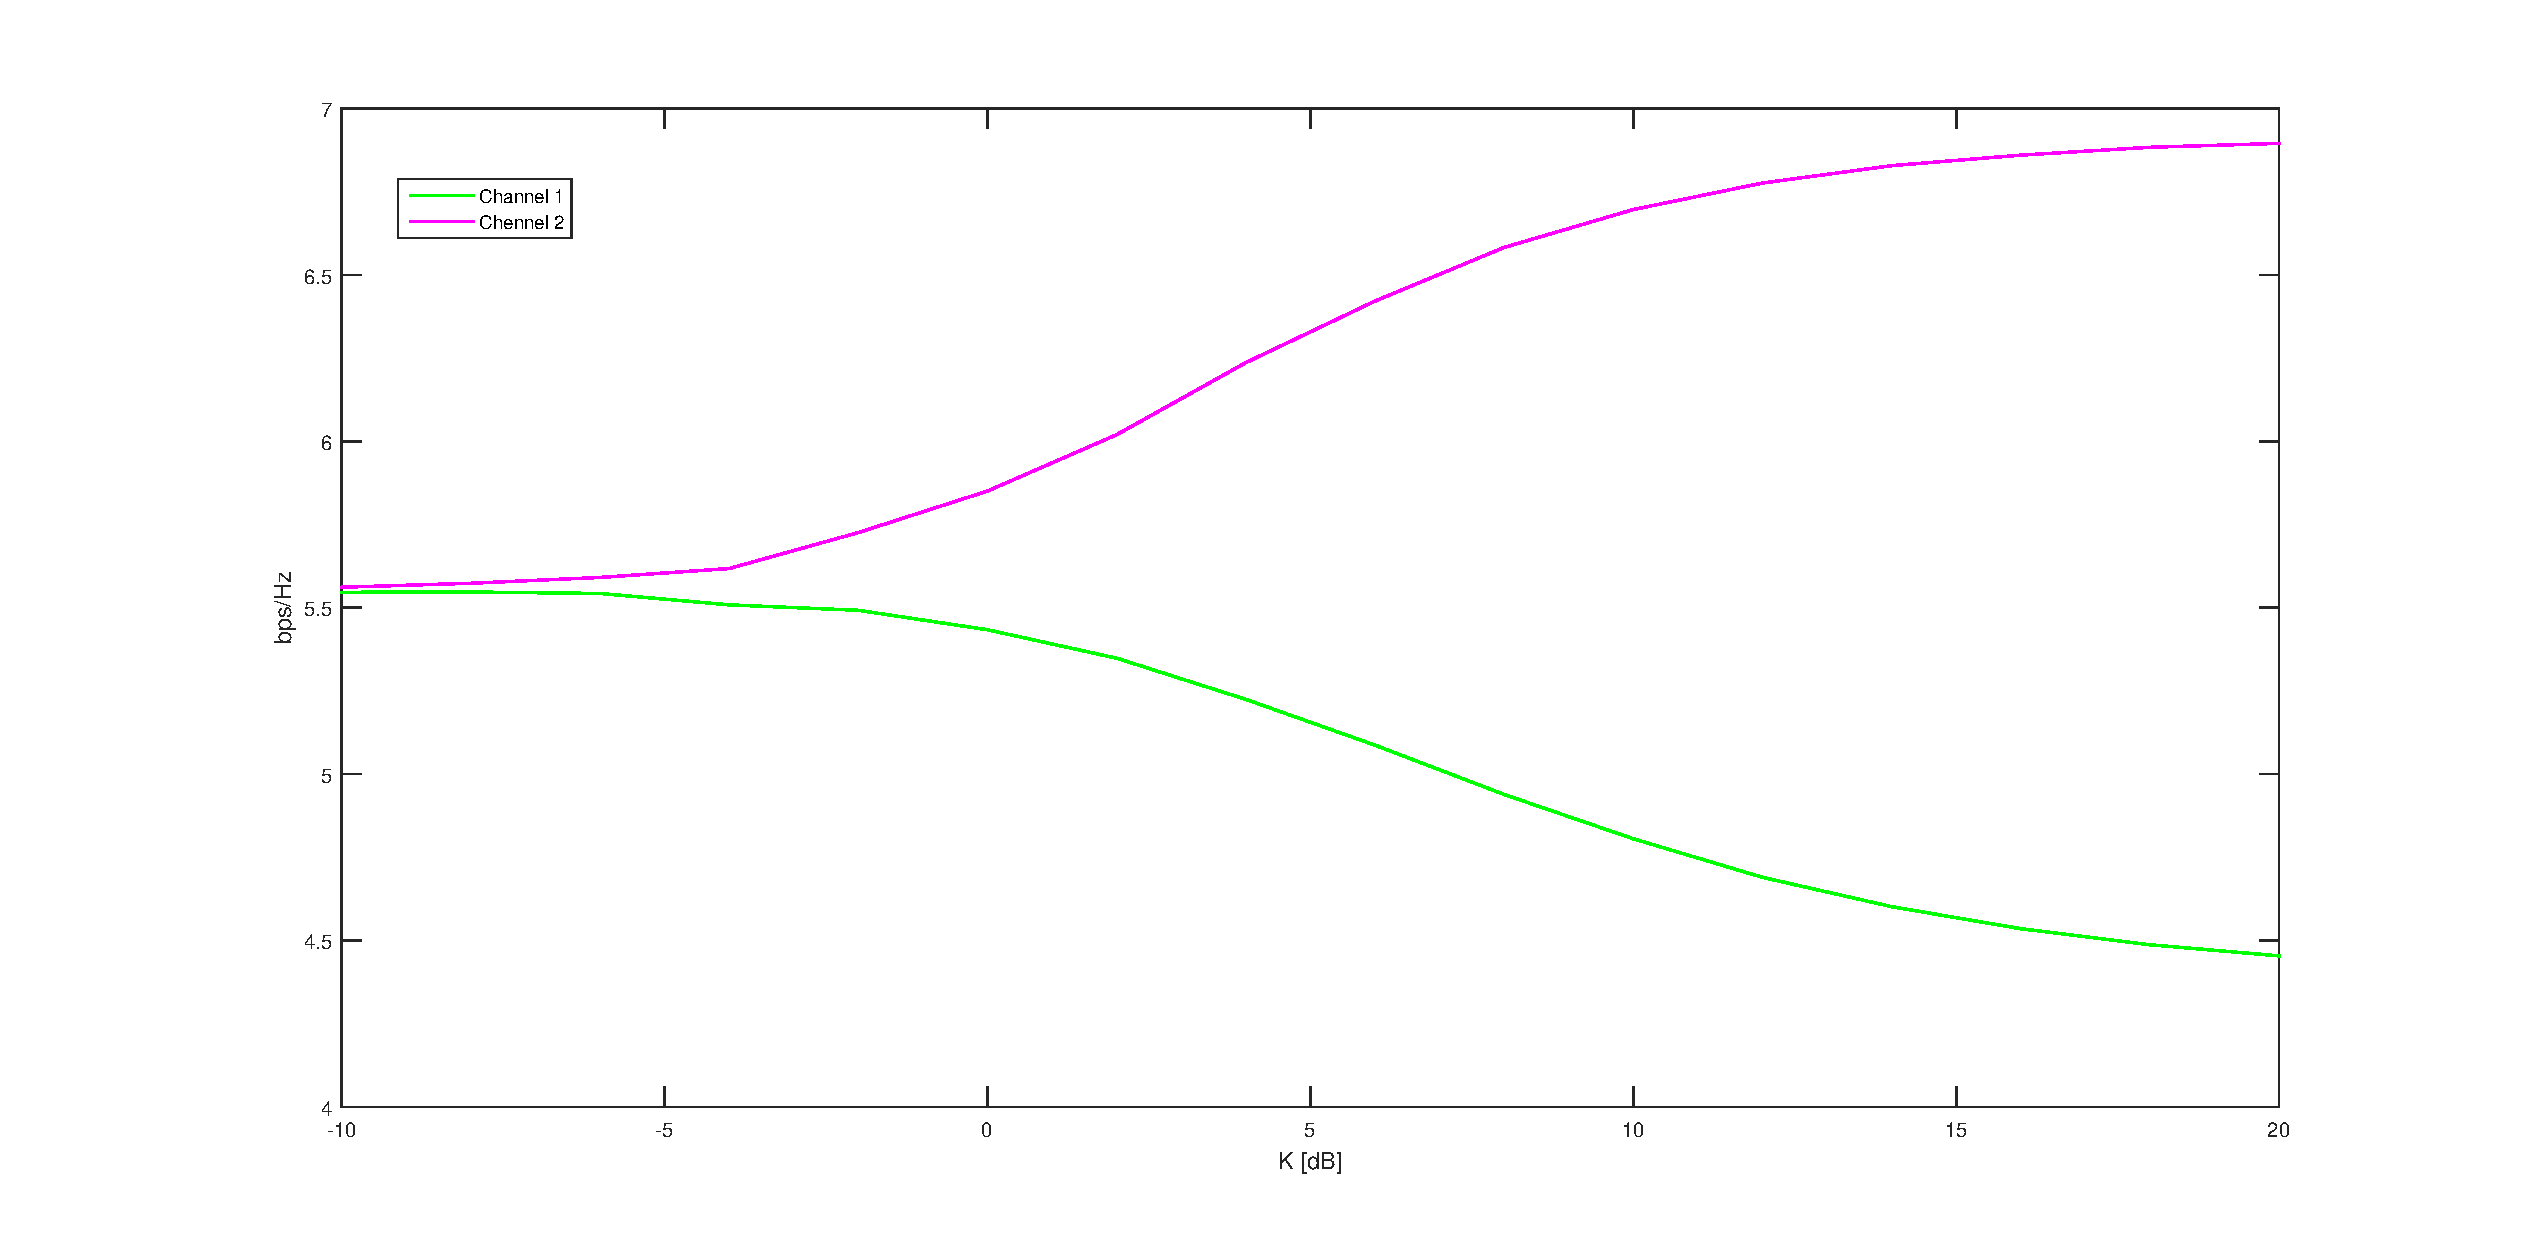
\includegraphics[width=6.0in]{mimoRic2.eps}\\
  \caption{Ergodic capacity vs K-factor for a MIMO channel with $H_1$ and $H_2$ LOS components.
The channel geometry has a significant impact on capacity at a high K-factor.}\label{fig:mimoRic2}
\end{figure}
\paragraph{Problem 7}
Find $XX^H$
\begin{eqnarray*}
{\bf X}{\bf X}^H &=& \left[
\begin{array}{cccc}
4 & 0 \\
0 & 4
\end{array}
\right]
\end{eqnarray*}
From the result we can conclude that {\bf X} is a orthogonal matrix.
\paragraph{Problem 8}
Let $x_1=1 + j$, $x_2=-1 + j$ and ${\bf h}=[h_1~~h_2]$ then
\begin{eqnarray*}
{\bf X} &=& \left[
\begin{array}{cccc}
x_1 & -x_2^* \\
x_2 & x_1^*
\end{array}
\right]=\left[
\begin{array}{cccc}
1+j & 1+j \\
-1+j & 1-j
\end{array}
\right]
\end{eqnarray*}
Received signal vector is ${\bf Y}=[y_1~~y_2^*]$, Where $$y_1=h_1x_1+h_2x_2$$ $$y_2=-h_1x_2^*+h_2x_1^*$$
Channel matrix is
\begin{eqnarray*}
{\bf H} &=& \left[
\begin{array}{cccc}
h_1 & h_2 \\
h_2^* & -h_1^*
\end{array}
\right]=\left[
\begin{array}{cccc}
0.2362 - 1.0244j & -0.3048 + 0.2587j \\
-0.3048 - 0.2587j & -0.3048 - 0.2587j
\end{array}
\right]
\end{eqnarray*}
We know $|{\bf h}|^2=1.2650$

$\tilde{{\bf X}}$ can be estimated as follows, $$\hat{{\bf X}}={\bf H^HY}$$
\begin{eqnarray*}
\hat{{\bf X}} &=& {\bf H^HY}=\left[
\begin{array}{cccc}
1 + j  \\
-1 + j 
\end{array}
\right]
\end{eqnarray*}
\paragraph{Problem 9} {\it (MISO array gain)} \quad
\begin{enumerate}
\item Applying the power constraint, we have $\mathcal E(\mathbf x^H \mathbf x)=2a^2<P$, so that the optimal gain is $a=\sqrt{P/2}$. The received signal for the MISO system is then $y=2as+n=\sqrt{2P}s+n$ with signal to noise ratio $\mathrm{SNR}_\text{MISO}=2P/N_0$.

The reference signal to noise ratio in a SISO system with transmit power $P$, channel gain $H=1$ and noise power $N_0$ is $\mathrm{SNR}_\text{SISO}=P/N_0$, and hence the MISO transmit array gain is $\mathrm{SNR}_\text{MISO} / \mathrm{SNR}_\text{SISO} = 2 = 3\,\text{dB}$.

\item In this case, the received signal is $y=-2as+n=-\sqrt{2P}s+n$, with $\mathrm{SNR}_\text{MISO}=2P/N_0$. Thus, the transmit array gain is still $3$\,dB.

\item With $h_1=1$,  $h_2=-1$ and $\mathbf x = a [s,s]^T$, the received signal is $y=n$. The signal to noise ratio is $0$, and thus array gain is $0=-\infty$\,dB. Not only do we get no transmit array gain, we are actually worse than the SISO system. This particular choice of transmit signal leads to cancellation of the desired signal.

With   $\mathbf x = s[a_1,a_2]^T$, the received signal is $y=(a_1-a_2)s+n$ with signal to noise ratio $(a_1-a_2)^2/N_0$. The power constraints evaluates to  $a_1^2+a_2^2\leq P$. To find the optimal $[a_1,a_2]$, solve the SNR maximization
\begin{align*}
	\text{maximize} &\quad (a_1-a_2)^2 / N_0\\
	\text{subject to} &\quad a_1^2+a_2^2\leq P.
\end{align*} 
This is a variant of the matched filtering problem. An optimal solution is $a_1=\sqrt{P/2}$ and $a_2=-\sqrt{P/2}$, which achieves the optimal value $\mathrm{SNR}_\text{MISO}=2P/N_0$, ths recovering the array gain $2=3$\,dB. Hence, transmit array gain is possible, but it requires channel knowledge at the transmitter. Only channel knowledge allows us to avoid signal cancellation and achieve coherent signal superposition.
\end{enumerate}

\paragraph{Problem 10}  {\it (Singular Values of $\mathbf H$) } 
The code for this problem is given:
\begin{footnotesize}
\verbatiminput{q2.m}
\end{footnotesize}
Fig. \ref{fig:min_eig} shows the distribution of the smallest
eigenvalue of ${\bf HH}^H$ using Monte Carlo simulations as well
as using the theoretical result.

One can derive a lower bound on the capacity of a MIMO channel
which is a function of the smallest eigenvalue only.  The
distribution of this lower bound thus depends on the pdf of the
smallest eigenvalue of ${\bf HH}^H$.

\begin{figure}[h]
  % Requires \usepackage{graphicx}
  \centering
  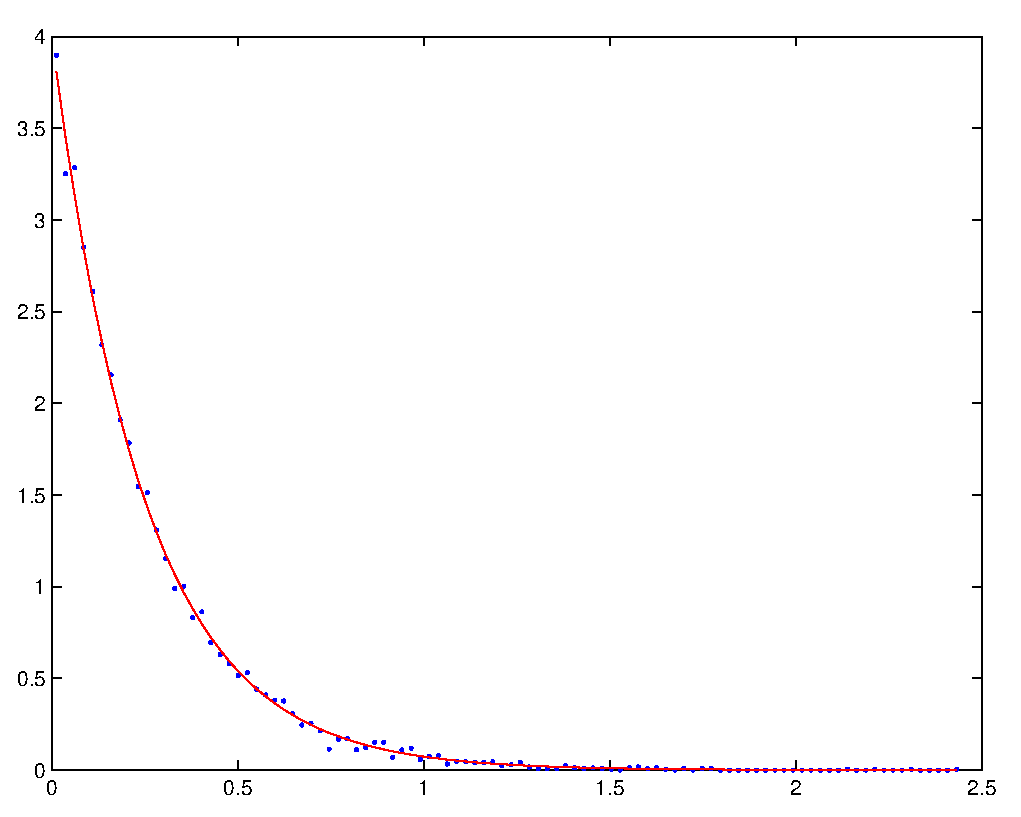
\includegraphics[width=4.0in]{min_eigenvalue.eps}\\
  \caption{Distribution of minimum eigenvalue of a $4\times 4$ $\bf{HH}^H$
  using both the formula (solid red) and simulation (blue dots)}\label{fig:min_eig}
\end{figure}








\end{document}

















